% You should not modify anything from here ... -------------
\documentclass[a4paper,12pt]{article}
\usepackage[english]{babel}
\usepackage{microtype,etex,listings,color,parskip}
\usepackage[margin=2cm]{geometry}
\usepackage{hyperref}
\lstset{
  language=Racket,
  tabsize=2,
  showstringspaces=false,
  breaklines=true,
  basicstyle=\ttfamily,
  keywordstyle=\color[rgb]{0.1,0.3,0.7}\ttfamily,
  stringstyle=\color[rgb]{0.7,0.1,0.3}\ttfamily,
  commentstyle=\color[rgb]{0.3,0.4,0.3}\ttfamily,
  columns=fixed,
  numberstyle=\sffamily\scriptsize,
  backgroundcolor=\color[rgb]{0.95,0.95,0.95},
  frame=lines,
  framexleftmargin=5pt,
  numbers = left,
  numberstyle = \footnotesize
}
% ... until here -------------------------------------------

\usepackage{graphicx}
\begin{document}

% replace X and XXX with the number and title of the assignment:
\title{El Despegue \\ Tarea 02}
% DO NOT ADD YOUR NAME, only your student numbers:
\author{Durazo Duarte Chelsea \\220216031}
\date{Lenguajes de programación 2022}

\maketitle


%%%%%%%%%%%%%%%%%%%%%%%%%%%%%%%%%%%%%%%%%%%%%%%%%%%%%%%%%%%%%%%%%%%
% NOTE: You MUST read and follow Appendix E of the lecture notes! %
%%%%%%%%%%%%%%%%%%%%%%%%%%%%%%%%%%%%%%%%%%%%%%%%%%%%%%%%%%%%%%%%%%%

\subsection*{Problema 5. La llamada (bundle ’(”a” ”b” ”c”) 0) es un buen uso de bundle? ¿qué produce?
¿por qué?}

\text{Solicitar a la función que empaquete un bufer el pedazos de longitud "0" no tiene sentido. Cuando hablamos de longitud esperamos una cantidad positiva y hablar de una longitud "0" haría referencia a algo inexistente, así la función \textit{bundle} se cicla. Esto sucede ya que la función drop no va reduciendo la lista y esta nunca llega al caso base cuando es vacía. \\
Sin embargo, al momento de programar es importante considerar todas las posibles entradas y asignar una salida por lo que consideré viable que en este caso la función devuelva una lista vacía.}



\subsection*{Problema 9.}

\begin{center}
    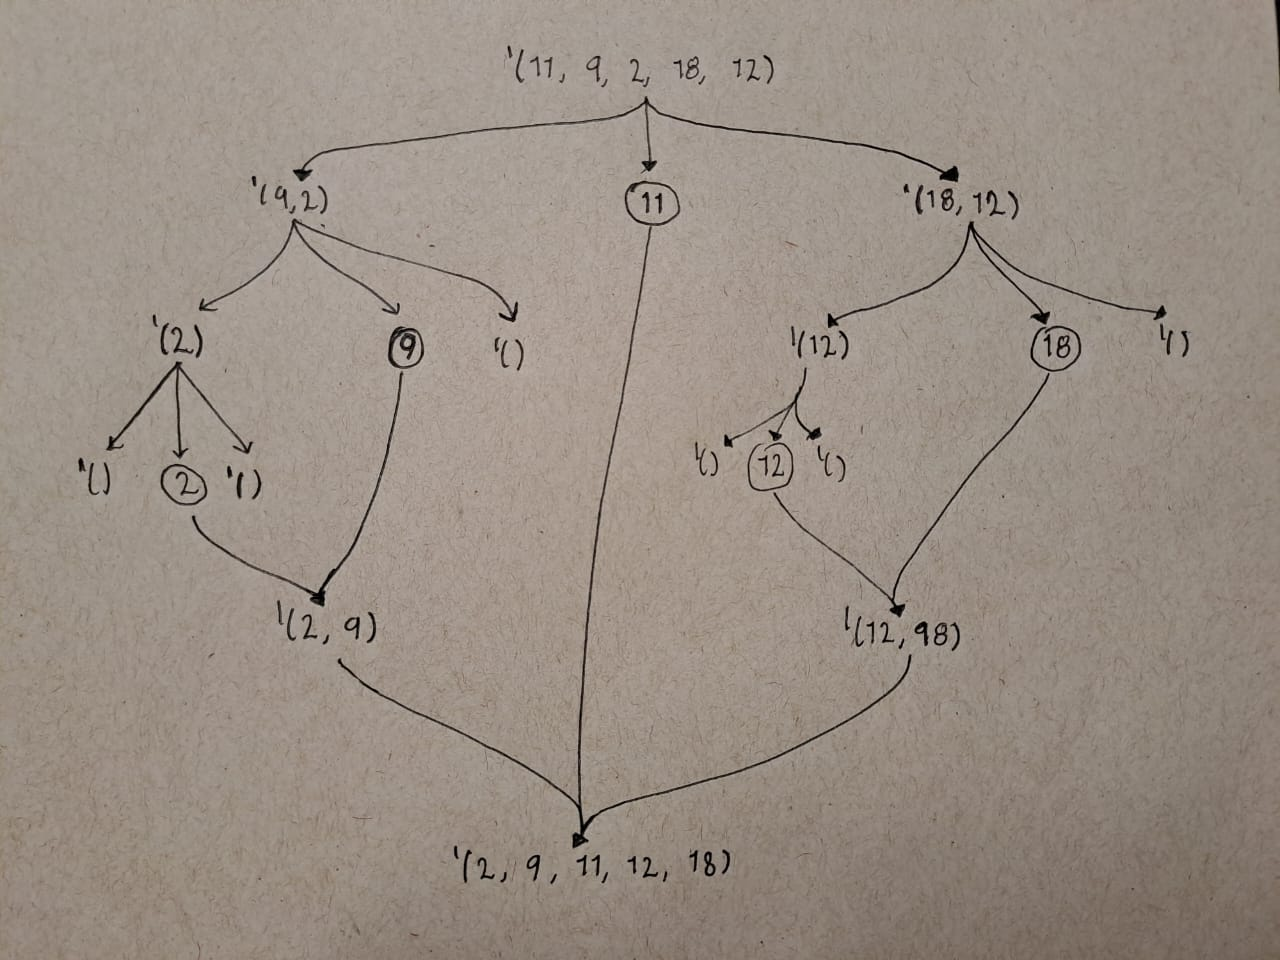
\includegraphics[scale=0.3]{arbol.png}
\end{center}


\subsection*{Problema 11. Si la entrada a quicksort contiene varias repeticiones de un número, va a regresar
una lista estrictamente más corta que la entrada. Responde el por qué y arregla el problema.}

\text{Sucede que solo se están considerando los elementos estrictamente mayores o menores que el pivote, por lo que todos los elementos iguales al pivote quedan fuera de la lista ordenada. La solución sería considerar en uno de los casos a los elementos menores/mayores e iguales al pivote, pero solo en uno de los casos.}


 \subsection*{Problema 13: Implementa una versión de quicksort que utilice isort si la longitud de la entrada está por debajo de un umbral. Determina este umbral utilizando la función time, escribe el procedimiento
que seguiste para encontrar este umbral}

\text{Implementé una función \textit{testing-sort} que verifica el tiempo dado según la función \textit{time} utilizando los dos algoritmos \textit{quicksort} y \textit{isort} para ordenar la misma lista.\\
La lista va creciendo multiplicando por 10 el anterior tamaño y en todos los casos el algoritmo \textit{quicksort} presenta un mejor desempeño, incluso hubo casos en los que en listas de menos de 50 elementos, \textit{quicksort} resultó ser más rápido.\\
Por lo anterior, el umbral del que habla el problema no existe. }


\subsection*{Problema 18. Considera la siguiente definición de smallers, uno de los procedimientos utilizados
en quicksort, responde en qué puede fallar al utilizar esta versión modificada en el procedimiento
de ordenamiento.
}
\lstinputlisting{smallers.rkt}

\text{a}


\subsection*{Problema 19. Describe con tus propias palabras cómo funciona find-largest-divisor de gcd-structural. Responde por qué comienza desde (min n m).}
\lstinputlisting{gcdstructural.rkt}

\text{EL algoritmo recorre uno a uno los elementos menores que el mínimo de los dos números dados tratando de encontrar el común divisor mayor entre los 2. Comienza desde el mínimo porque el máximo común divisor es, como máximo, el menor de los dos números.}

\subsection*{Problema 20. Describe con tus propias palabras cómo funciona find-largest-divisor de gcd-generative.}
\lstinputlisting{gcdgenerative.rkt}

\text{En este caso se toma como máximo posible común divisor el residuo que queda de dividir el mayor entre el menor si no lo es el menor, lo que resulta en una búsqueda mucho más rápida.}


\subsection*{Problema 21.: Utiliza la función time para determinar cuál de las dos implementaciones es más eficiente, escribiendo tu respuesta con los tiempos de ejecución obtenidos con ambos procedimientos para valores “pequeños”, “medianos” y “grandes”. Justifica qué valores usaste en cada una de estas mediciones y por qué los consideraste de ese “tamaño”.}

\text{Utilizé como valores pequeños, números menores a 1000 cuya diferencia con su máximo común divisor sea la máxima, para valores medianos utilicé la misma premisa con números menores de 1000000, y para números muy grandes, menores a 1000000000.\\
Después de las pruebas determiné que el algoritmo más eficiente sería el generativo. Los números fueron asignados de ese tamaño porque con números mayores ya tardaba mucho en terminar el algoritmo.}

\begin{figure}[htb]
    \centering
    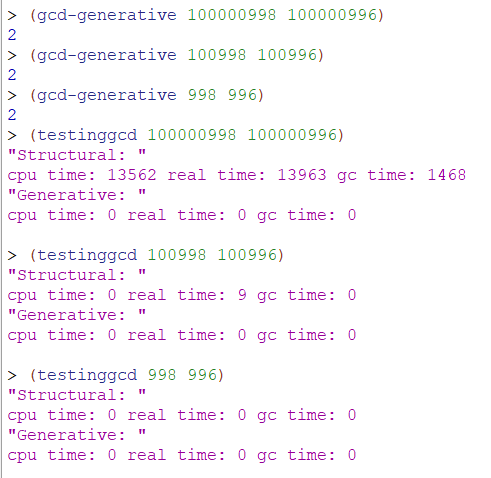
\includegraphics{gcd.png}
\end{figure}


\subsection*{Problema 22. Piensa y describe por qué no siempre es la mejor opción elegir el procedimiento más eficiente en tiempo de ejecución. Utiliza criterios que no sean el de “eficiencia”.}


\text{En ocasiones es importante priorizar otros aspectos, tales como el uso de memoria, o en proyectos grandes es importante la legibilidad del procedimiento. Así el mejor procedimiento se designaría según la importancia que se le de a cada uno de los aspectos según el contexto.}



% \section{Appendix: test cases} % Optional
%
% ...

% \section{Appendix: Extensions} % Optional
%
% ...

\end{document}
